\section{Data Debugging: Spreadsheets}
\label{sec:evaluation}

\begin{figure*}[!t]
\centering
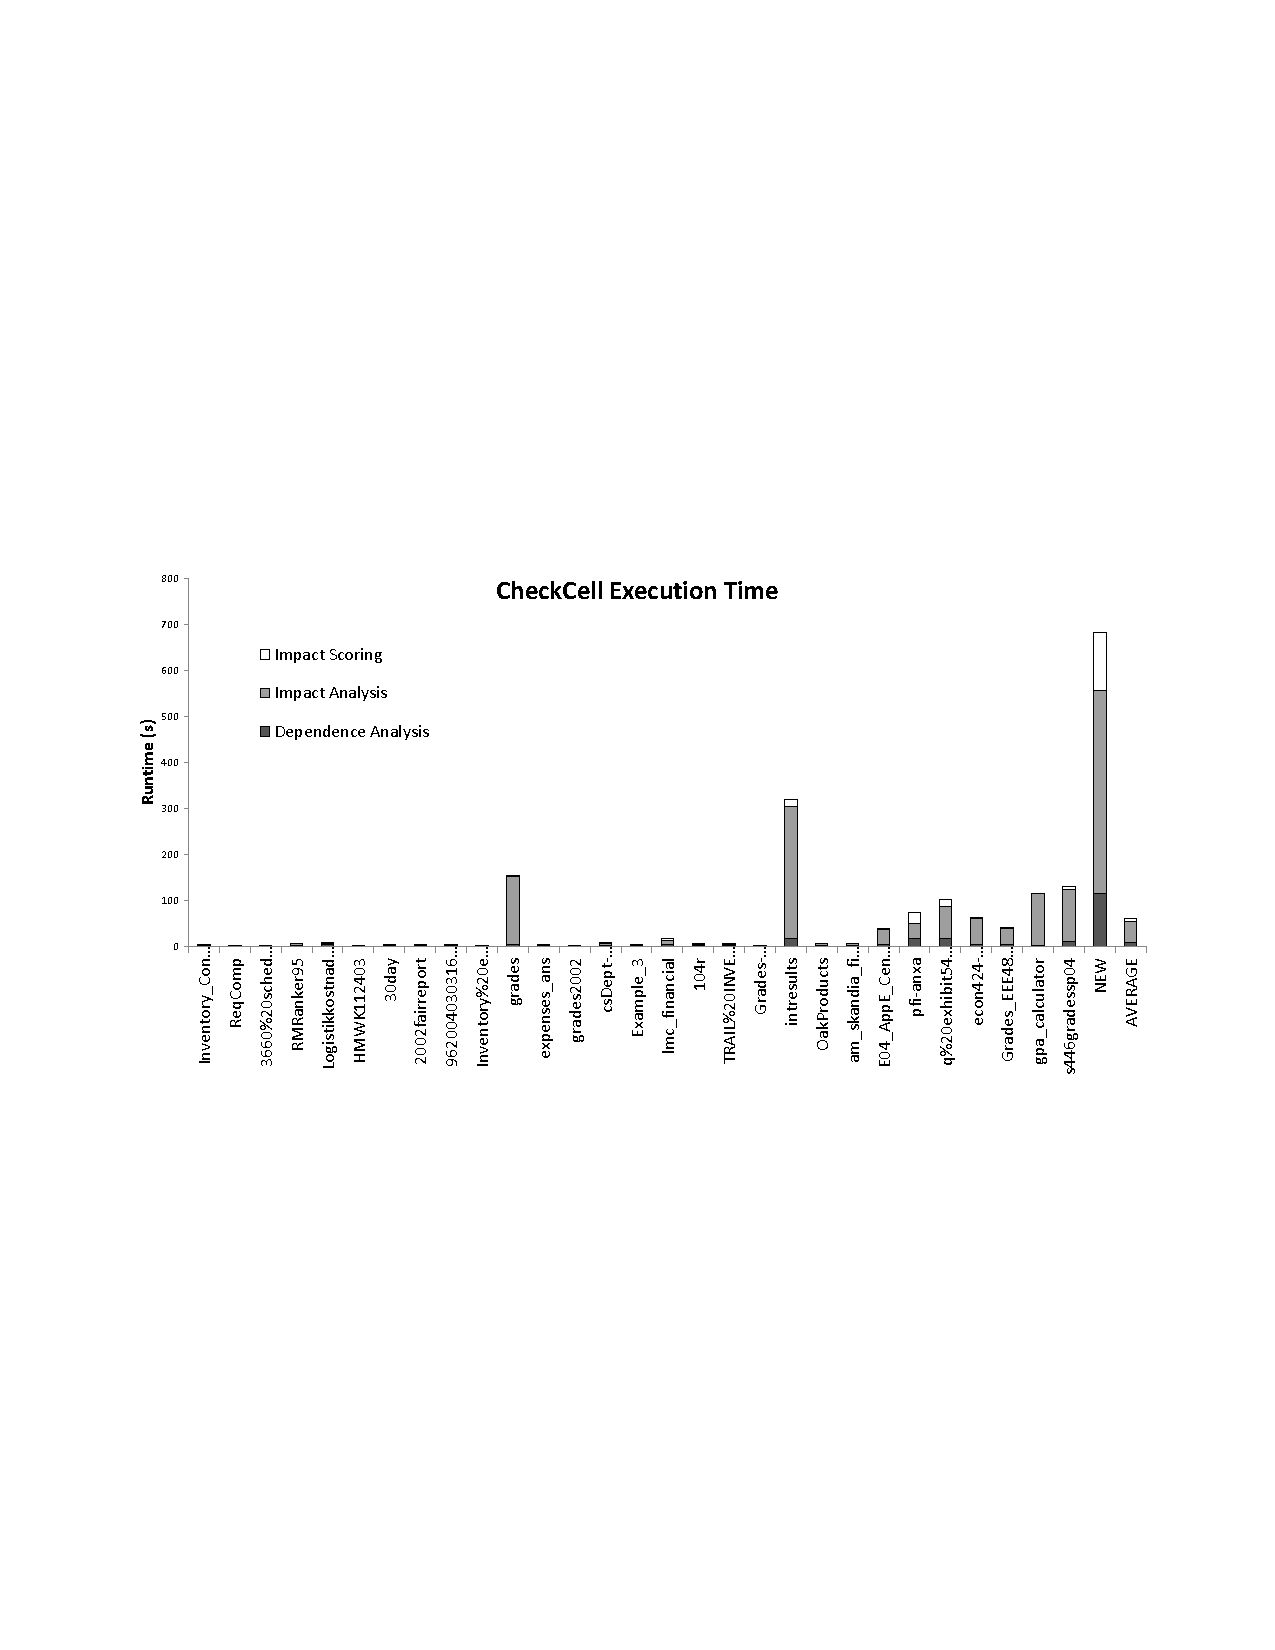
\includegraphics[width=5.5in]{execution_time_graph}
  \caption{\checkcell{} execution time. For most of the spreadsheets, \checkcell{} completes its analysis in under 9 seconds; for all but two, it completes in under three minutes.\label{fig:execution_time_graph}}
\end{figure*}
 
\punt{
\begin{table*}[!b]
  \centering \begin{tabular}{l|rrr||r|rrr}
 \small{\bf{Spreadsheet}} & \small{\bf{Formulas}} & \small{\bf{Cells}} & \small{\bf{Cells}} & \small{\bf{Runtime}} & \small{\bf{Dep.}} & \small{\bf{Impact}}   & \small{\bf{Impact}} \\
 & & {\small{\it{raw}}} & {\small{\it{weighted}}} & \small{\it{total (s)}} & \small{\bf{Analysis}} & \small{\bf{Analysis}} & \small{\bf{Scoring}} \\
\hline
\small{3660 schedule S2003} & \small{31} & \small{1} & \small{0} & \small{1.54} & \small{0.73} & \small{0.44} & \small{0.34} \\ 
\small{ReqComp} & \small{54} & \small{162} & \small{0} & \small{1.95} & \small{0.95} & \small{0.52} & \small{0.44} \\ 
\small{Inventory\_Control} & \small{33} & \small{21} & \small{0} & \small{4.71} & \small{1.67} & \small{1.59} & \small{1.42} \\ 
\small{RMRanker95} & \small{79} & \small{54} & \small{11} & \small{7.07} & \small{2.74} & \small{2.38} & \small{1.91} \\ 
\small{Logistikkostnader} & \small{73} & \small{29} & \small{26} & \small{8.88} & \small{3.48} & \small{2.97} & \small{2.40} \\  
\small{HMWK112403} & \small{36} & \small{41} & \small{27} & \small{2.31} & \small{0.88} & \small{0.78} & \small{0.63} \\ 
\small{30day} & \small{125} & \small{92} & \small{30} & \small{3.01} & \small{1.39} & \small{1.31} & \small{0.27} \\ 
\small{2002fairreport} & \small{3} & \small{39} & \small{39} & \small{4.30} & \small{1.29} & \small{1.67} & \small{1.30} \\ 
\small{9620040303160820} & \small{42} & \small{81} & \small{81} & \small{4.77} & \small{1.19} & \small{2.74} & \small{0.81} \\  
\small{Inventory errors} & \small{100} & \small{129} & \small{90} & \small{2.83} & \small{1.25} & \small{1.02} & \small{0.53} \\ 
\small{grades} & \small{227} & \small{661} & \small{96} & \small{154.45} & \small{3.06} & \small{149.85} & \small{1.51} \\ 
\small{expenses\_ans} & \small{57} & \small{60} & \small{120} & \small{3.24} & \small{0.92} & \small{2.15} & \small{0.15} \\ 
\small{grades2002} & \small{61} & \small{143} & \small{123} & \small{2.67} & \small{1.03} & \small{1.11} & \small{0.51} \\ 
\small{csDept-PayrollTimecardEntry} & \small{68} & \small{204} & \small{124} & \small{7.37} & \small{1.85} & \small{4.37} & \small{1.10} \\  
\small{Example\_3} & \small{71} & \small{130} & \small{127} & \small{3.15} & \small{1.22} & \small{1.56} & \small{0.28} \\ 
\small{lmc\_financial} & \small{72} & \small{148} & \small{142} & \small{17.15} & \small{4.69} & \small{7.63} & \small{4.80} \\ 
\small{104r} & \small{22} & \small{146} & \small{144} & \small{6.66} & \small{1.81} & \small{3.26} & \small{1.54} \\ 
\small{TRAIL INVENTORY N\#A850A} & \small{2} & \small{156} & \small{156} & \small{6.15} & \small{1.12} & \small{3.99} & \small{0.99} \\ 
\small{Grades-6\_excerpt} & \small{106} & \small{168} & \small{168} & \small{1.83} & \small{1.10} & \small{0.45} & \small{0.25} \\ 
\small{intresults} & \small{1066} & \small{3158} & \small{239} & \small{318.91} & \small{17.12} & \small{287.63} & \small{14.12} \\ 
\small{OakProducts} & \small{69} & \small{271} & \small{242} & \small{6.82} & \small{1.67} & \small{4.20} & \small{0.91} \\ 
\small{am\_skandia\_fin\_supple\#A80EE} & \small{56} & \small{272} & \small{268} & \small{6.64} & \small{1.53} & \small{4.01} & \small{1.06} \\ 
\small{E04\_AppE\_Census\_Database\_50} & \small{42} & \small{300} & \small{300} & \small{39.04} & \small{4.07} & \small{32.72} & \small{2.22} \\ 
\small{pfi-anxa} & \small{5} & \small{310} & \small{310} & \small{73.56} & \small{16.38} & \small{33.10} & \small{24.05} \\ 
\small{q exhibit54-OEA} & \small{797} & \small{1160} & \small{365} & \small{102.56} & \small{18.03} & \small{68.70} & \small{15.79} \\ 
\small{econ424-fall2003-publ\#A8A23} & \small{93} & \small{517} & \small{384} & \small{62.83} & \small{3.91} & \small{56.96} & \small{1.93} \\ 
\small{Grades\_EEE481\&581} & \small{177} & \small{757} & \small{756} & \small{40.11} & \small{3.31} & \small{35.74} & \small{1.03} \\ 
\small{gpa\_calculator} & \small{80} & \small{80} & \small{819} & \small{115.86} & \small{1.88} & \small{113.67} & \small{0.28} \\ 
\small{s446gradessp04} & \small{335} & \small{1369} & \small{1247} & \small{129.36} & \small{9.76} & \small{113.29} & \small{6.27} \\ 
\small{NEW} & \small{2626} & \small{2574} & \small{2403} & \small{683.32} & \small{115.75} & \small{440.30} & \small{127.23} \\ 
    \end{tabular}%
  \caption{The benchmark suite of 30 spreadsheets, a random sample from the EUSES repository~\cite{Fisher:2005:ESC:1082983.1083242}, ordered by weighted number of cells. The raw number of cells indicates the total number of cells that are used in any formula; the weighted number of cells weighs cells \emph{in ranges} by the number of formulas that depend on it. A breakdown of \checkcell{} execution times (in seconds) appears on the right side.\label{tab:spreadsheet_characteristics}}
\end{table*}
}

In our preliminary work, we have developed the \checkcell{} prototype
for data debugging in spreadsheets.  \checkcell{} runs as an add-in in
Microsoft Excel 2010, and incorporates the algorithms described in the
overview. Figure~\ref{fig:personal_budget_highlighted} shows the
effect of running \checkcell{} on the example described above, which
in this case identifies cell \texttt{B4} as the only one with an
unusual impact on the spreadsheet.


We evaluate \checkcell{} analytically and empirically across
two dimensions: its execution time, and its effectiveness at finding
actual errors. 
%  Our
%experimental platform is a 13'' MacBook Air equipped 4GB of RAM and an
%Intel Core i5-2557M processor running at 1.70GHz. The operating system
%is Windows 7 Professional (SP1), which executes non-virtualized (via
%Bootcamp).

\subsection{Runtime: Analysis}
\label{sec:asymptotic_analysis}

Data debugging operates in several phases: computing the dependence
graph, performing impact analysis, and then ranking impacts. Runtime
depends on the following parameters: the number of data items ($n$),
the number of formulas ($f$), and the number of inputs ($i$). In
spreadsheets, the number of inputs equals the number of data items,
but in other contexts like databases, inputs correspond to fields, so
$i \ll n$. Since each formula and data item must be examined at least
once to compute the dependence graph and to measure impact,
respectively, runtime for data debugging must be 
$\Omega(n+f)$.

The cost of building the dependence graph varies depending on the
structure of the computation. It has a worst-case runtime of
$O((i*f)^2)$, quadratic in the total number of inputs and formulas; it
is theoretically possible for each formula to depend on every input
and other formula. However, this kind of pathological computation
structure is atypical. Dependence graphs normally form a tree or a
forest of trees. In this case, the cost of constructing the dependence
graph becomes linear in the number of inputs and formulas, or
$O(i+f)$.

Impact analysis dominates the costs of constructing the dependence
graph and ranking impacts, since it requires recalculation of the
computations affected by changes in the data.

A na\"ive implementation of impact analysis that checked the impact of
each data item by systematically replacing it with every other item in
the same range would require $O(n^2)$ time. Worse, each of these
iterations requires potentially costly recalculations. For large
ranges, such an approach would make data debugging unusable in
practice.
 
By using a fixed number of random selections once the range
exceeds a threshold size, data debugging keeps the total number of
recalculations to $O(n)$, linear in the number of data items. Any
strategy that visits each data item at least once takes $O(n)$ time,
so this bound is tight.

Finally, ranking impacts involves only two linear passes over the
impacts to compute absolute impact scores, so it also operates in
(optimal) linear time in the number of impacts.

\subsection{Runtime: Empirical Results}

To empirically measure the runtime of \checkcell{}, we run it on a random subset
of 30 spreadsheets drawn from the EUSES
corpus~\cite{Fisher:2005:ESC:1082983.1083242}, excluding those that do not contain
formulas.

Figure~\ref{fig:execution_time_graph} reports the performance of data
debugging across our spreadsheet suite, ordered by the weighted number
of cells.

For 19 of the 30 spreadsheets, \checkcell{} takes 9 seconds or less to
complete. Its runtime is less than three minutes for all but two of
the spreadsheets: \texttt{intresults} and \texttt{NEW}, which take 318
seconds and 683 seconds, respectively. The average runtime over all
spreadsheets is 61 seconds; without the two outliers, it is 29
seconds. The cost of \checkcell{} is generally proportional to the
cost of the impact analysis, which is in turn dependent on the
weighted number of cells.

The spreadsheets that require the most execution time both have by far
the largest number of formulas (1,066 and 2,626), and the latter also
has the largest number of weighted cells (2,403). Their relatively
high execution time is attributable to the fact that the cost of impact
analysis increases as the number of formulas increases, since the
Excel recalculation engine must do more work per item tested. The
\texttt{intresults} spreadsheet also has an extremely highly-connected
clique in its dependence graph, which leads to both higher time for
dependence analysis and increases the cost of recalculations during
impact analysis. % (see Figure~\ref{fig:intresults_tree}).

%\paragraph{Summary:} For nearly every spreadsheet
% examined, \checkcell{}'s runtime is under three minutes.

% Info about the benchmarks.

% \subsection{Benchmarks}

%\subsection{Case Studies}

% \paragraph{9-Grades}

\subsection{Error Detection: Empirical Results}
\label{sec:user_study}

While \checkcell{} can be used across the EUSES suite, looking for
errors in existing spreadsheets is problematic because we do not know
what the ground truth is. To evaluate \checkcell{}'s efficacy at
finding actual errors, we need errors and ground truth to compare it
against.

Rather than artificially inject errors, we designed an experiment that
allows us to observe real errors produced by people and use
\checkcell{} to find them. We collect human errors by hiring workers
to perform data entry tasks (entering known data) via Amazon's
Mechanical Turk, a popular crowdsourcing platform, and then check
their results with \checkcell{}.

Our ground truth data is drawn from \texttt{3q2000.xls}, a
spreadsheet from the EUSES repository that contains selected financial
information from Fannie Mae. We save the data as a comma-separated
value file (.csv). Mechanical Turk workers were paid 3 cents to
enter 10 of these numerical values at a time into a web form designed to look
like a spreadsheet, shown in Figure~\ref{fig:mturk_task}. To prevent
copying and pasting, we generate an image containing the
comma-separated values. Each worker had the opportunity to perform up
to seven different tasks.

In all, we collected 200 responses from 46 distinct users. Out of
these responses, 14 had omitted data and 52 contained errors, for an
overall error rate of 33\%. The errors can be classified into the following categories:

\begin{itemize}
\item \textbf{Sign omission}, where a negative sign was dropped;
\item \textbf{Magnitude errors}, any change in a value (usually a dropped or spurious digit) that results in an order of magnitude increase or decrease;
\item \textbf{Digit transposition}, where at least two digits are transposed;
\item \textbf{Typos}, any other typographical error (e.g., a mistyped digit).
\end{itemize}

We then inserted the erroneous data back into the spreadsheet one at a
time and ran \checkcell{} to see whether it found any of these
errors. Recall that by design, \checkcell{} reports data with an
unusual impact on any of the calculations. For this
spreadsheet, \checkcell{} always highlights the values in the top row
(the net interest income) because these values have a significant
impact on the spreadsheet; most of the income in this spreadsheet
comes from this row. We classify \checkcell{} as having correctly
found an error if it also highlights an erroneous cell.

For 13 of the 52 erroneous inputs (25\%), \checkcell{} correctly marks
the cell with the error, supporting our hypothesis that locating data
with unusual impact also finds errors. In all but two of these cases,
the error was a magnitude error; such errors are likelier to have an
unusual impact on a computation than all other errors, since they
change the input data dramatically. Even sign omission only causes a
factor of two change in a data element. Nonetheless, 20 of the errors
that \checkcell{} does not report also involve magnitude errors, but
those errors occur in data that do not contribute significantly to any
computation.


\begin{figure*}[!t]
\centering
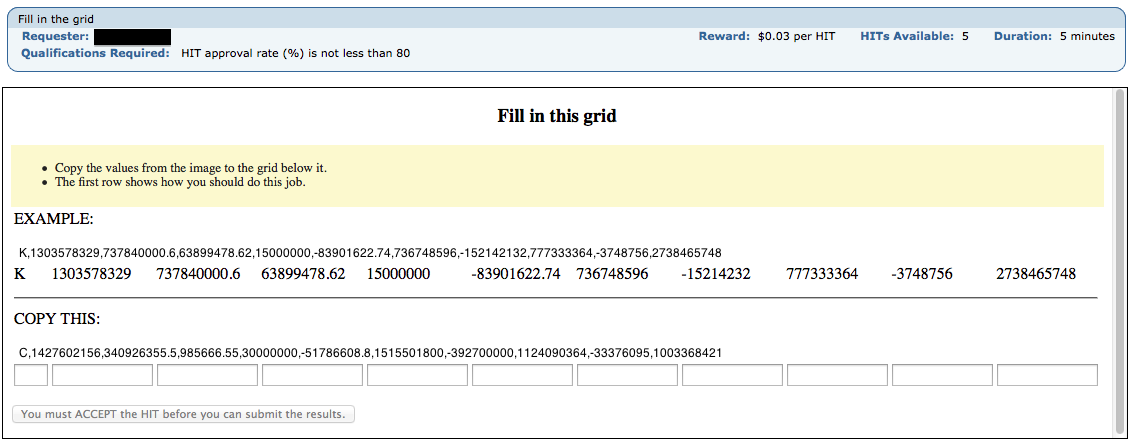
\includegraphics[width=5.5in]{images/mturk_fuzz_task}
  \caption{The page presented to Mechanical Turk workers to perform data entry tasks in order to collect actual human data entry errors (see Section~\ref{sec:user_study}).\label{fig:mturk_task}}
\end{figure*}


\begin{figure*}[!t]
\centering
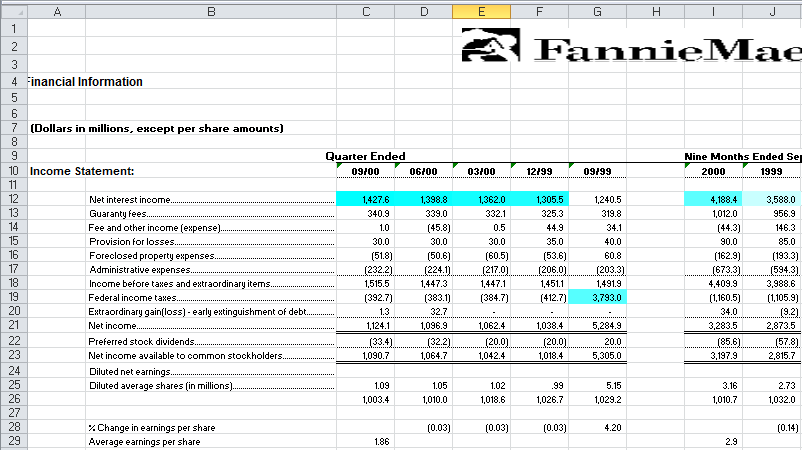
\includegraphics[width=5.5in]{images/fannie_mae_outlier}
  \caption{A screenshot of \checkcell{}'s results. In addition to the top row, which has a large impact on the final results, \checkcell{} highlights cell \texttt{G19}, a human data entry error.\label{fig:fannie_mae}}
\end{figure*}

Figure~\ref{fig:fannie_mae} presents a screenshot of \checkcell{}'s
results with one of these errors. In addition to the top
row, \checkcell{} indicates that cell \texttt{G19} has an unusual
impact; this is, in fact, the error. The correct value
for \texttt{G19} is \texttt{-379300000}, and the value entered by the
worker was \texttt{3793000000}: the worker made both a sign error and
an order of magnitude error (one too many 0's).

\paragraph{Summary:} By searching for data with unusual impacts on the spreadsheet, \checkcell{} is able to successfully find actual human data entry errors.

\subsection{Proposed Work}

We plan to improve the performance of data debugging in spreadsheets
by applying static analysis. The primary component of \checkcell{}'s
overhead is the cost of recomputation during sampling. By peeling back
the black box assumption and applying analysis to the actual formulas
involved in the computation, it is possble to compute a data item's
impact directly, without having to perform sampling and repeated
re-computations.

For example, consider a formula that computes the sum of the cells A1
through A10. Our current approach would find the influence of each of
the cells by replacing each cell by one of the other cells in the
range, and thus would perform 90 computations. However, the impact of
each cell $A_i$ can be computed equivalently in the following way
without the need for any substitutions as $\sum_{j=1}^{10}{A_j} -
(\frac{10}{9})(\sum_{j=1}^{10}{A_j} - A_i)$.  By storing the result of the first
sum, it is possible to efficiently compute the impact of each $A_i$,
with no need for sampling.

Many of the most commonly used functions in Excel are as well-behaved
as the SUM function. These include average, standard deviation, and
most counting functions. When a computation consists entirely of these
functions, it will be possible to dramatically reduce the cost of data
debugging. Of course, computations contain functions that are not
well-behaved, or whose computation is not possible to analyze because
it is a user-defined compiled function. Nonetheless, it will be
possible to speed data debugging whenever formulas consist of
well-behaved functions combined with other functions using operations
like addition. We plan to handle dependent chains of functions by
effectively inlining the functions into their parents and then performing
analysis and simplification on that larger function.

